\chapter{Diseño} \label{diseño}

\section{Arquitectura del sistema}
Para abordar la estructuración y diseño del sistema, se ha optado por una arquitectura que asegure la escalabilidad, la resiliencia y la mantenibilidad. Con este objetivo, se ha decidido implementar una arquitectura basada en microservicios con el frontend desacoplado. Esta decisión permitirá dividir la lógica de negocio en servicios individuales e independientes, facilitando buenas prácticas de desarrollo y  la evolución del sistema.

\begin{figure}[H]
    \centering
    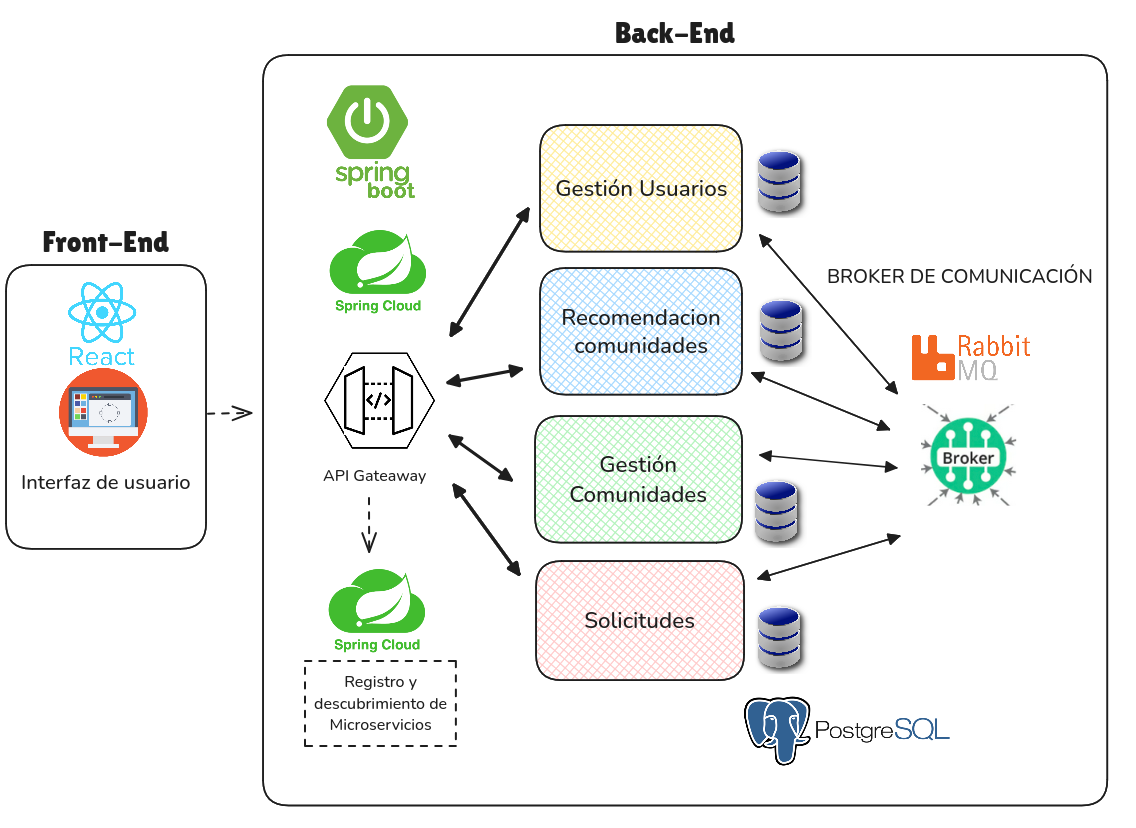
\includegraphics[width=0.95\textwidth]{fotos/diagrama-sistema.png}
    \caption{Diagrama de la arquitectura del sistema.}
    \label{fig:arq}
\end{figure}
\section{Arquitectura del Backend}
El back-end del sistema estará basado en una \textbf{arquitectura de microservicios} \cite{richardsonMicroservices}. Esta decisión responde a las ventajas que ofrece este estilo arquitectónico  en términos de modularidad, escalabilidad y mantenimiento. Sin embargo, es importante tener en cuenta que este tipo de estilo arquitectónico, también implica una mayor complejidad en términos de creación y comunicación entre los servicios. A continuación, se expondrán las características fundamentales que seguirá nuestra estructura definida en la figura \ref{fig:arq}.

\subsection{Estructura de los Microservicios}


\begin{itemize}
    \item \textbf{Microservicios Independientes:} Cada microservicio es responsable de un conjunto de funcionalidades relacionadas, que constituyen una parte lógica del sistema.
    \item \textbf{Base de Datos Independiente:} Cada microservicio tiene su propia base de datos, lo que permite un aislamiento completo de sus datos y mejora la resiliencia del sistema.
    \item \textbf{Comunicación Asíncrona:} La comunicación entre microservicios se realiza a través de un broker de mensajería \textbf{RabbitMQ} \cite{RabbitMQ}, basado en eventos. Esto permite mantener la asincronía en las operaciones, lo cual mejora la eficiencia y la escalabilidad.
    \item \textbf{API Gateway:} Para facilitar la comunicación entre el frontend y los microservicios, se implementará una \textbf{API Gateway}. Este componente será responsable de verificar los tokens de autenticación y enrutará las solicitudes al microservicio adecuado. Además, la API Gateway proporcionará un punto único de entrada para el frontend, simplificando el acceso a los servicios backend.
\end{itemize}


\subsection{Estructura Interna de los Microservicios}
Dentro de cada microservicio se ha seguido una arquitectura basada en capas, en general es muy cercana al Modelo-Vista-Controlador a excepción de que en este caso, la vista se estructura de forma completamente aislada. Como se observa en la imagen \ref{fig:capas}, en la estructura del sistema encontramos las siguientes capas:

\begin{itemize}
    \item \textbf{Capa de Datos:} En ella se definen las entidades que serán mapeadas a la base de datos. Estas entidades representan los objetos de dominio del microservicio.
    \item \textbf{Capa de Presentación:} Se encarga de definir las operaciones de la API del microservicio. Define las rutas, valida las solicitudes y delega la lógica del sistema a la capa de negocio.
    \item \textbf{Capa de Negocio:} Contiene la lógica de negocio. Aquí se implementan las operaciones del sistema interactuando con la capa de datos para realizar operaciones en la base de datos.
\end{itemize}
\begin{figure}[h!]
    \centering
    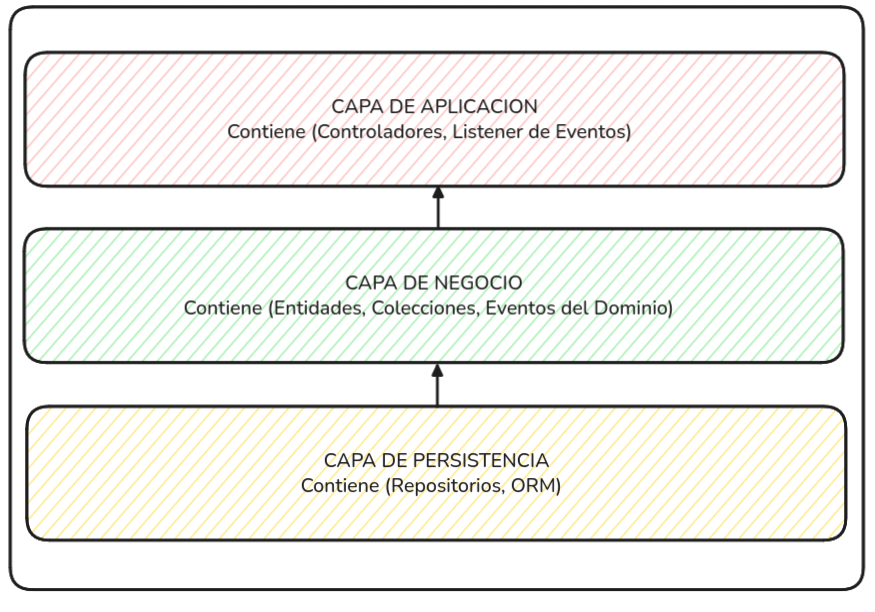
\includegraphics[width=\textwidth]{fotos/capas-backend.png}
    \caption{Diagrama de la arquitectura del backend}
    \label{fig:capas}
\end{figure}

\section{Arquitectura del Frontend}
Para el frontend se ha seguido una arquitectura conocida como \textbf{Scream Architecture}, la cual nace del concepto de Clean Code \cite{martin_clean_architecture} que busca mejorar la organización de los proyectos software asegurando que tanto el diseño como el código comuniquen claramente su intención.

\subsection{Scream Architecture}
La \textbf{Scream Architecture} se basa en organizar el código de manera que cada dominio o característica de la aplicación tenga su propia estructura de carpetas. Como vemos en la imagen \ref{fig:scream}, esto permite sustituir la clásica agrupación por componentes, por una arquitectura que facilita la mantenibilidad, escalabilidad del código y facilidad de entendimiento.

\begin{figure}[H]
    \centering
    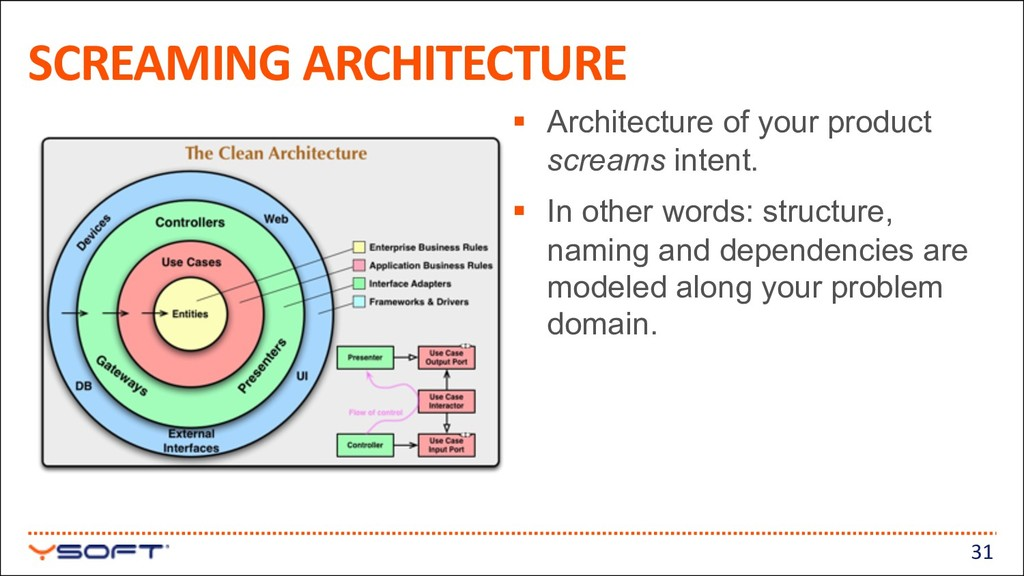
\includegraphics[width=\textwidth]{fotos/explication-screaming.jpg}
    \caption{Explicación arquitectura screaming. Fuente: \cite{speakerdeck_screaming}}
    \label{fig:scream}
\end{figure}

\subsection{Estructura de la Carpeta Feature}
Siguiendo la filosofía de esta arquitectura, nuestro frontend tiene un directorio \texttt{feature} que contiene diferentes subcarpetas para cada dominio del sistema. Por ejemplo, si se tiene un dominio \textit{usuario}, dentro del directorio \texttt{usuario} se organizarán todos los archivos relacionados con ese dominio, tales como: Login del usuario, Registro del usuario y sus respectivos formularios. Para cada feature encontraremos las siguientes carpetas:


\begin{itemize}
    \item \textbf{API Calls}: Se configuran las funciones que realizan las llamadas a la API del back-end relacionadas con la entidad \texttt{usuario}.
    \item \textbf{Types/Interfaces}: Se definen los tipos de datos utilizados en la entidad, como las interfaces de los objetos \texttt{usuario}.
    \item \textbf{Pages}: Se configuran las páginas o vistas relacionadas con esa entidad, organizadas dentro de la misma carpeta para mantener el código ordenado.
    \item \textbf{Components}: Si la entidad necesita componentes específicos, estos también se colocan dentro de su carpeta correspondiente.
\end{itemize}

Esta estructura permite que cada entidad se gestione de forma aislada y autónoma dentro del proyecto, lo que facilita la localización de funcionalidades y el mantenimiento de cada módulo.


\section{Descripción de la API de cada microservicio}
Como se mencionó anteriormente, el back-end estará compuesto por una serie de microservicios, cada uno encargado de encapsular una parte específica de la lógica de negocio del sistema. Cada microservicio expondrá una API que ofrecerá las distintas operaciones del sistema. A continuación, se va a mostrar los distintos endpoints que compondrán la API de cada microservicio.


\subsection{Microservicio Gestión de Usuarios}

\begin{tcolorbox}[colback=blue!5!white, colframe=blue!75!black, title=\texttt{/usuarios/} -- POST]
\textbf{Descripción:} Registra un nuevo usuario en el sistema. \\
\textbf{Body (DTO):} \texttt{UsuarioDTO} : Nombre de usuario, contraseña, correo, LifestyleDTO \\
\textbf{Salida:} \texttt{token JWT} \\
\textbf{Respuesta:}
\begin{itemize}[label=--]
    \item 201 Created: Usuario creado exitosamente.
    \item 400 Bad Request: Datos inválidos o usuario ya existe.
\end{itemize}
\end{tcolorbox}

\vspace{0.5em}

\begin{tcolorbox}[colback=blue!5!white, colframe=blue!75!black, title=\texttt{/usuario/login} -- POST]
\textbf{Descripción:} Autenticación de un usuario. \\
\textbf{Body:}
\begin{itemize}[label=--]
    \item Nombre de usuario.
    \item Contraseña.
\end{itemize}
\textbf{Salida:} \texttt{token JWT} \\
\textbf{Respuesta:}
\begin{itemize}[label=--]
    \item 200 OK: Autenticación correcta.
    \item 400 Bad Request: Credenciales inválidas.
\end{itemize}
\end{tcolorbox}

\vspace{0.5em}

\begin{tcolorbox}[colback=blue!5!white, colframe=blue!75!black, title=\texttt{/usuarios/} -- GET]
\textbf{Descripción:} Devuelve todos los Usuarios contenidos en el sistema. \\
\textbf{Salida:} \texttt{Lista de usuarios} \\
\textbf{Respuesta:}
\begin{itemize}[label=--]
    \item 200 OK: Usuarios encontrados.
    \item 404 Not Found: No hay usuarios.
\end{itemize}
\end{tcolorbox}

\vspace{0.5em}

\begin{tcolorbox}[colback=blue!5!white, colframe=blue!75!black, title=\texttt{/usuario/delete/\{id-usuario\}} -- POST]
\textbf{Descripción:} Elimina un usuario específico. \\
\textbf{Parámetro:} \texttt{id-usuario} (URL path) \\
\textbf{Respuesta:}
\begin{itemize}[label=--]
    \item 204 No Content: Usuario eliminado.
    \item 500 Internal Server Error: Fallo al eliminar.
\end{itemize}
\end{tcolorbox}

\vspace{0.5em}

\begin{tcolorbox}[colback=blue!5!white, colframe=blue!75!black, title=\texttt{/usuario/\{id-usuario\}} -- PATCH]
\textbf{Descripción:} Actualiza los datos de un usuario concreto. \\
\textbf{Body (DTO):} \texttt{Campos a modificar del UsusarioDTO} \\
\textbf{Parámetro:} \texttt{id-usuario} (URL path) \\
\textbf{Respuesta:}
\begin{itemize}[label=--]
    \item 200 OK: Usuario modificado.
    \item 404 Not Found / 500 Internal Server Error: Error.
\end{itemize}
\end{tcolorbox}

\vspace{0.5em}

\begin{tcolorbox}[colback=blue!5!white, colframe=blue!75!black, title=\texttt{/usuario/\{id-usuario\}} -- GET]
\textbf{Descripción:} Obtiene los datos de un usuario específico. \\
\textbf{Salida (DTO):} \texttt{UsuarioDTO} \\
\textbf{Parámetro:} \texttt{id-usuario} (URL path) \\
\textbf{Respuesta:}
\begin{itemize}[label=--]
    \item 200 OK: Usuario encontrado.
    \item 404 Not Found: No existe el usuario.
\end{itemize}
\end{tcolorbox}


\subsection{Microservicio Gestión de Comunidades}
\begin{tcolorbox}[title=\texttt{GET /comunidades}, colback=blue!5!white, colframe=blue!75!black]
\textbf{Descripción:} Devuelve todas las comunidades disponibles. \\
\textbf{Salida:} \texttt{Lista de comunidades} \\
\textbf{Respuesta:}
\begin{itemize}[label=--]
    \item \textbf{202 Accepted} – Comunidades encontradas.
    \item \textbf{500 Internal Server Error} – Error interno al obtener los datos.
\end{itemize}
\end{tcolorbox}

%-------------------------------
\begin{tcolorbox}[title=\texttt{GET /comunidades/\{id-comunidad\}}, colback=blue!5, colframe=blue!80!black]
\textbf{Descripción:} Devuelve los datos de una comunidad específica.

\textbf{Parámetro:} \texttt{id-comunidad} (URL path) \\
\textbf{Salida:} \texttt{ComunidadDTO}\\
\textbf{Respuesta:}
\begin{itemize}[label=--]
    \item \textbf{202 Accepted} – Comunidad encontrada.
    \item \textbf{404 Not Found} – Comunidad no encontrada.
\end{itemize}
\end{tcolorbox}

%-------------------------------
\begin{tcolorbox}[title=\texttt{POST /comunidades/}, colback=blue!5!white, colframe=blue!80!black]
\textbf{Descripción:} Registra una nueva comunidad.

\textbf{Body – ComunidadDTO:}
\begin{itemize}[label=--]
    \item \texttt{nombre}: String  
    \item \texttt{descripcion}: String  
    \item \texttt{localizacion}: String  
    \item \texttt{preferencias}: String
    \item \texttt{idAdmin}: Long
\end{itemize}

\textbf{Respuesta:}
\begin{itemize}[label=--]
    \item \textbf{202 Accepted} – Comunidad creada (devuelve ID).
    \item \textbf{500 Internal Server Error} – Error al crear comunidad.
\end{itemize}
\end{tcolorbox}

%-------------------------------
\begin{tcolorbox}[title=\texttt{PATCH /comunidades/\{id-comunidad\}}, colback=blue!5, colframe=blue!80!black]
\textbf{Descripción:} Modifica los datos de una comunidad existente.

\textbf{Parámetro:} \texttt{id-comunidad} (URL path) \\

\textbf{Body – ComunidadDTO:}
\begin{itemize}[label=--]
    \item \texttt{nombre,descripción,localización,preferencias}.
\end{itemize}

\textbf{Respuesta:}
\begin{itemize}[label=--]
    \item \textbf{202 Accepted} – Comunidad modificada.
    \item \textbf{500 Internal Server Error} – Error al modificar.
\end{itemize}
\end{tcolorbox}

%-------------------------------
\begin{tcolorbox}[title=\texttt{DELETE /comunidades/delete/\{id-comunidad\}}, colback=blue!5, colframe=blue!80!black]
\textbf{Descripción:} Elimina una comunidad existente.

\textbf{Parámetro:} \texttt{id-comunidad} (URL path) \\

\textbf{Respuesta:}
\begin{itemize}[label=--]
    \item \textbf{202 Accepted} – Comunidad eliminada correctamente.
    \item \textbf{400 Bad Request} – Error al borrar la comunidad.
\end{itemize}
\end{tcolorbox}

\begin{tcolorbox}[title=\texttt{POST /comunidades/\{id-comunidad\}/usuarios/\{id-usuario\}/}, colback=blue!5, colframe=blue!80!black]
\textbf{Descripción:} Añade un usuario a la comunidad.

\textbf{Parámetros:}
\begin{itemize}[label=--]
    \item \texttt{Id de la comunidad}: Id de la comunidad
    \item \texttt{Id del usuario}: Id del usuario a añadir.
\end{itemize}

\textbf{Respuesta:}
\begin{itemize}[label=--]
    \item \textbf{200 Accepted} – Usuario añadido correctamente.
    \item \textbf{400 Bad Request} – Error al añadir usuario a la comunidad.
\end{itemize}
\end{tcolorbox}


\begin{tcolorbox}[title=\texttt{DELETE /comunidades/\{id-comunidad\}/usuarios/\{id-usuario\}}, colback=blue!5, colframe=blue!80!black]
\textbf{Descripción:} Elimina un usuario de la comunidad.

\textbf{Parámetro:}
\begin{itemize}[label=--]
    \item \texttt{id-comunidad}: Id de la comunidad a la que pertenece el usuario a eliminar
    \item \texttt{id-usuario}: Id del usuario a eliminar.
\end{itemize}

\textbf{Respuesta:}
\begin{itemize}[label=--]
    \item \textbf{200 Accepted} – Usuario eliminado de la comunidad correctamente.
    \item \textbf{400 Bad Request} – Error al eliminar la comunidad.
\end{itemize}
\end{tcolorbox}

\begin{tcolorbox}[title=\texttt{GET /comunidades/\{id-comunidad\}/tareas}, colback=blue!5, colframe=blue!80!black]
\textbf{Descripción:} Devuelve las tareas asociadas a una comunidad específica.

\textbf{Parámetro:} \texttt{Id de la comunidad} (URL path) \\
\textbf{Salida (Lista):} \texttt{Tareas}

\textbf{Respuesta:}
\begin{itemize}[label=--]
    \item \textbf{202 Accepted} – Tareas encontradas.
    \item \textbf{404 Not Found} – Comunidad no encontrada.
\end{itemize}
\end{tcolorbox}

\begin{tcolorbox}[title=\texttt{GET /comunidades/\{id-comunidad\}/eventos/}, colback=blue!5, colframe=blue!80!black]
\textbf{Descripción:} Devuelve los eventos asociados a una comunidad específica.

\textbf{Parámetro:} \texttt{id-comunidad} (URL path) \\
\textbf{Salida (Lista):} \texttt{Eventos} 

\textbf{Respuesta:}
\begin{itemize}[label=--]
    \item \textbf{202 Accepted} – Eventos encontrados.
    \item \textbf{404 Not Found} – Comunidad no encontrada.
\end{itemize}
\end{tcolorbox}

\begin{tcolorbox}[title=\texttt{GET /comunidades/\{id-comunidad\}/tareas/\{id-usuario\}/}, colback=blue!5, colframe=blue!80!black]
\textbf{Descripción:} Devuelve las tareas asociadas a una comunidad y usuario específico.

\textbf{Parámetro:}
\begin{itemize}[label=--]
    \item \texttt{id-comunidad}: Comunidad a obtener los datos (String)
    \item \texttt{id-usuario}: Usuario a obtener los datos (String)
\end{itemize}
\textbf{Salida (Lista):} \texttt{Tareas}

\textbf{Respuesta:}
\begin{itemize}[label=--]
    \item \textbf{202 Accepted} – Tareas encontradas.
    \item \textbf{404 Not Found} – Comunidad/Usuario no encontrada.
\end{itemize}
\end{tcolorbox}
\subsection{Recomendación de Comunidades}
%-------------------------------
\begin{tcolorbox}[title=\texttt{GET /usuarios/\{id-usuario\}/recomendaciones}, colback=blue!5, colframe=blue!80!black]
\textbf{Descripción:} Busca las comunidades afines al usuario y las devuelve de forma ordenada.

\textbf{Parámetro:} \texttt{id-usuario} (URL path) \\
\textbf{Lógica:}
Se calcula las comunidades afines con una función interna, calcularRecomendacion.\\
\textbf{Salida (Lista):} \texttt{Comunidades}\\
\textbf{Respuesta:}
\begin{itemize}[label=--]
    \item \textbf{202 Accepted} – Devuelve una Lista de Comunidades afines
    \item \textbf{400 Bad Request} – Error al calcular las comunidades.
\end{itemize}
\end{tcolorbox}

\begin{tcolorbox}[title=\texttt{GET /usuarios/\{id-usuario\}/recomendaciones/filtrado}, colback=blue!5, colframe=blue!80!black]
\textbf{Descripción:} Busca las comunidades afines al usuario y les aplica el filtro seleccionado.

\textbf{Parámetro:} \texttt{id-usuario} (URL path) \\
\textbf{Entrada:}
\begin{itemize}[label=--]
    \item \texttt{Filtros a aplicar (Distancia, precio, número de integrantes}.
\end{itemize}
\textbf{Lógica:}
Se calcula las comunidades afines con una función interna, calcularRecomendacion. Entre esas comunidades se descartan las que no pasan el filtro.\\
\textbf{Salida (Lista):} \texttt{Comunidades}\\
\textbf{Respuesta:}
\begin{itemize}[label=--]
    \item \textbf{202 Accepted} – Devuelve una Lista de Comunidades afines filtradas.
    \item \textbf{400 Bad Request} – Error al calcular las comunidades.
\end{itemize}
\end{tcolorbox}

\subsection{Solicitudes}

\begin{tcolorbox}[title=\texttt{GET /usuarios/\{id-usuario\}/solicitudes}, colback=blue!5, colframe=blue!80!black]
\textbf{Descripción:} Obtiene las solicitudes de un usuario concreto.

\textbf{Parámetro:} \texttt{id-usuario} (URL path) \\
\textbf{Salida (Lista):} \texttt{Solicitudes}\\

\textbf{Respuesta:}
\begin{itemize}[label=--]
    \item \textbf{202 Accepted} – Devuelve todas las solicitudes del usuario
    \item \textbf{400 Bad Request} – Error al encontrar las solicitudes del usuario.
\end{itemize}
\end{tcolorbox}
\begin{tcolorbox}[title=\texttt{POST /usuarios/\{id-usuario\}/solicitudes}, colback=blue!5, colframe=blue!80!black]
\textbf{Descripción:} Crea una nueva solicitud.

\textbf{Body:}
\begin{itemize}[label=--]
    \item \texttt{Id del usuario destinatario}
    \item \texttt{Mensaje a enviar con la solicitud}
\end{itemize}

\textbf{Respuesta:}
\begin{itemize}[label=--]
    \item \textbf{200 Accepted} – Solicitud creada correctamente.
    \item \textbf{400 Bad Request} – Error al crear la solicitud.
\end{itemize}
\end{tcolorbox}

\section{Diagrama Entidad-Relación}
El diagrama de Entidad-Relación permitirá representar de forma visual la relación entre las entidades del sistema contenidas en la base de datos. Esto permitirá visualizar los atributos que componen cada entidad y las relaciones entre ellas.
\begin{figure}[H]
    \centering
    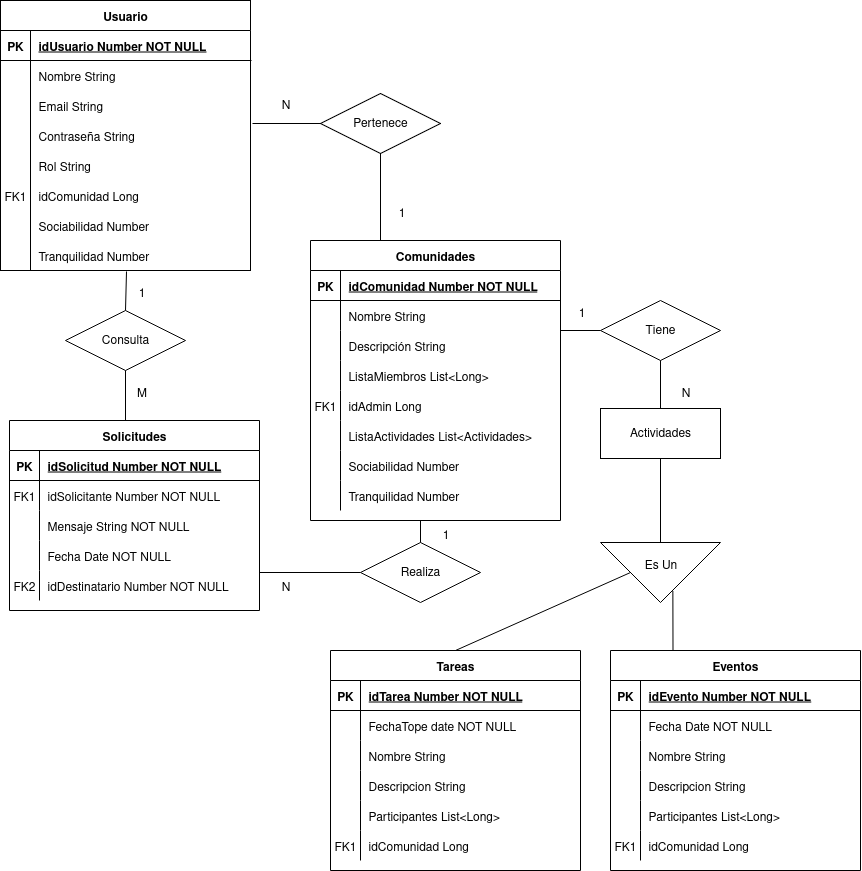
\includegraphics[width=\textwidth]{fotos/er-final.png}
    \caption{Diagrama de Entidad-Relación del sistema.}
    \label{fig:er-final}
\end{figure}
\newpage
\section{Diagrama de Clases}
El diagrama de clases muestra los distintos atributos de las entidades del sistema junto a sus operaciones y relaciones. Esto  permitirá crear un mapa conceptual del sistema entendiendo que debe realizar cada entidad y como se relacionan entre ellas.

\begin{figure}[H]
    \centering
    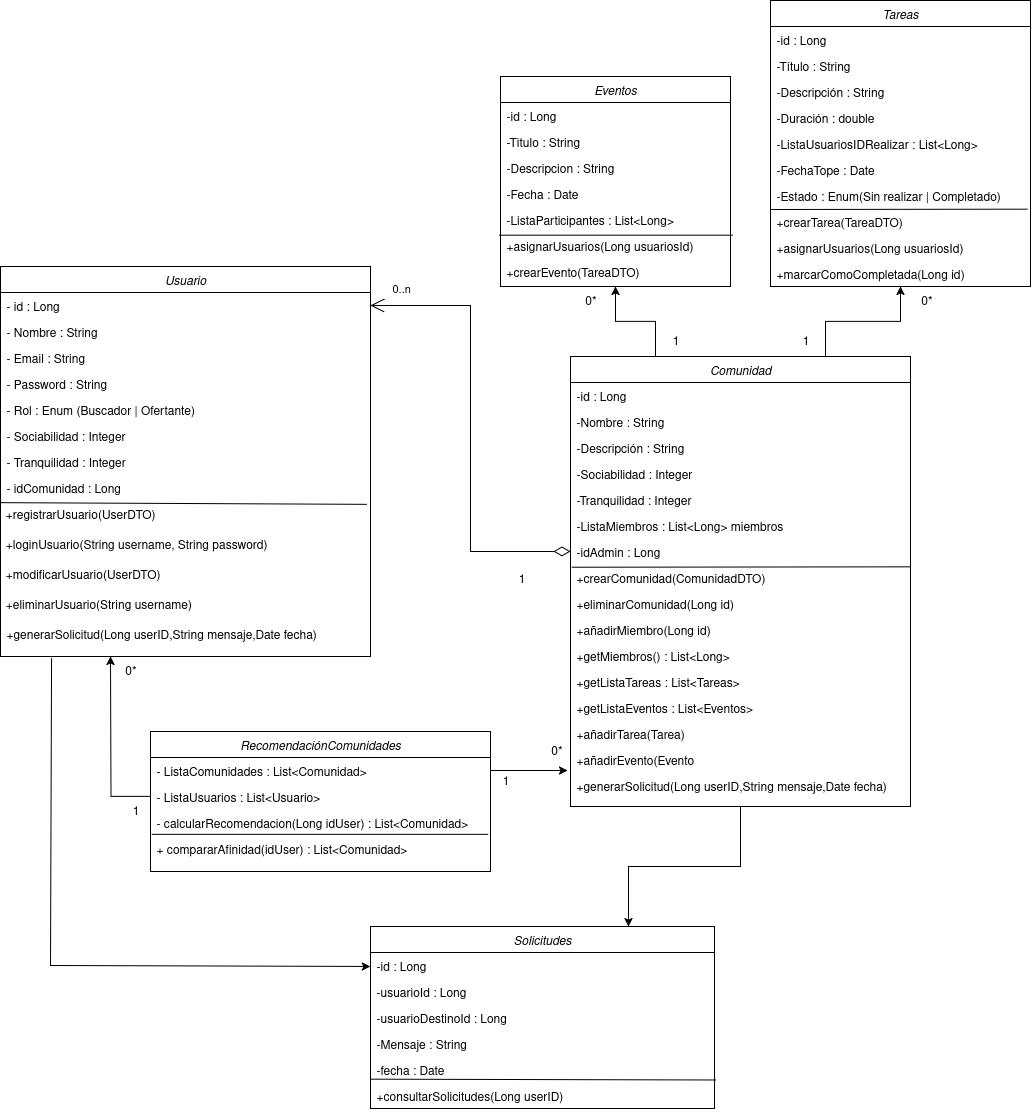
\includegraphics[width=1\textwidth]{fotos/UML5.png}
    \caption{Diagrama UML de entidades del sistema.}
\end{figure}

\section{Diagramas de Secuencia}
Con el objetivo de ilustar la implementación de los métodos más relevantes del sistema, se llevará a cabo los diagramas de secuencia de las siguientes operaciones: Registro de usuario, Inicio de sesión, Unión a comunidad, Búsqueda de Comunidad, Consultar Tareas, Reparto de tareas y Crear Tarea.

\begin{figure}[H]
    \centering
    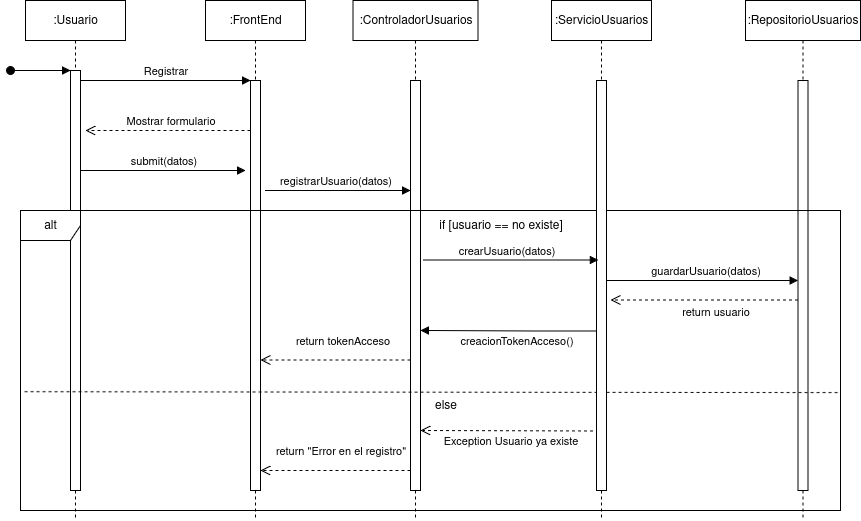
\includegraphics[width=\textwidth]{fotos/1-secuencia.png}
    \caption{Diagrama de secuencia del registro.}
    \label{fig:diagrama_arquitectura}
\end{figure}

\begin{figure}[H]
    \centering
    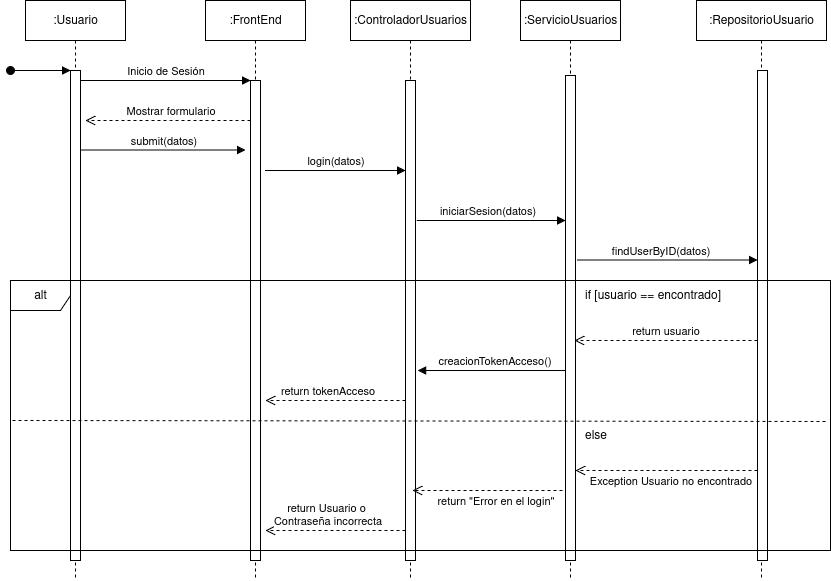
\includegraphics[width=\textwidth]{fotos/2-secuencia.png}
    \caption{Diagrama de secuencia del login.}
    \label{fig:diagrama_arquitectura}
\end{figure}
\begin{figure}[H]
    \centering
    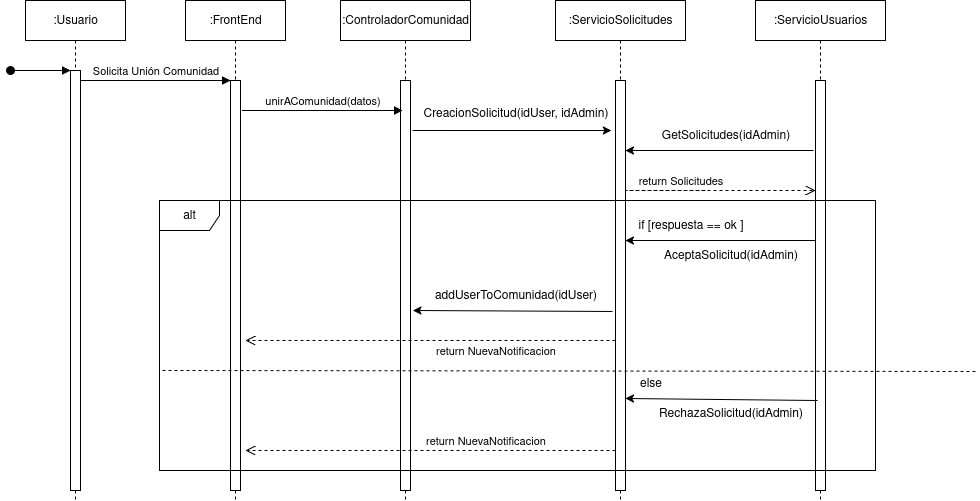
\includegraphics[width=1\textwidth]{fotos/3-secuencia.png}
    \caption{Diagrama de secuencia unión a una comunidad.}
    \label{fig:diagrama_arquitectura}
\end{figure}

\begin{figure}[H]
    \centering
    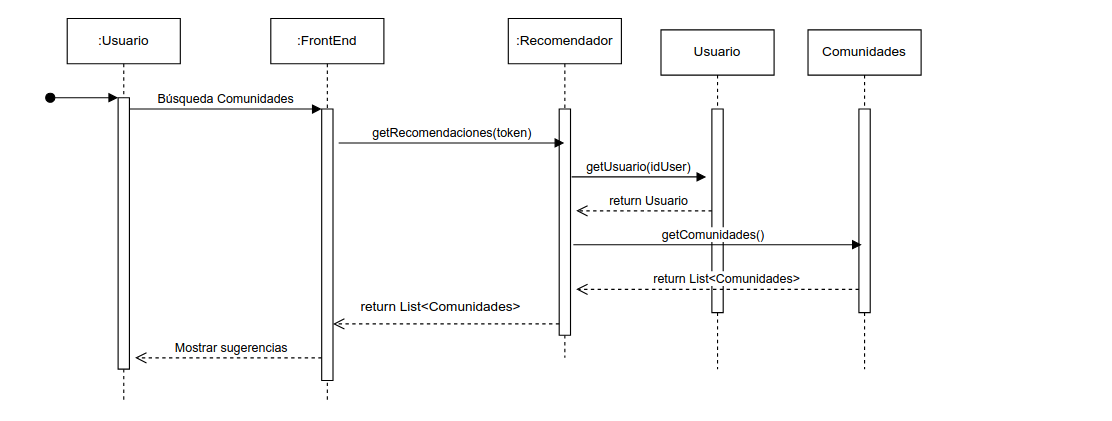
\includegraphics[width=1\textwidth]{fotos/4-secuencia.png}
    \caption{Diagrama de secuencia búsqueda de comunidades.}
    \label{fig:diagrama_arquitectura_2}
\end{figure}

\begin{figure}[H]
    \centering
    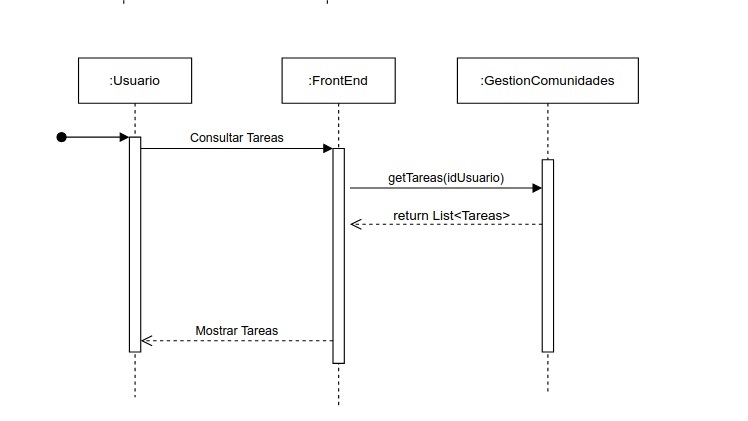
\includegraphics[width=\textwidth]{fotos/5-secuencia.png}
    \caption{Diagrama de secuencia consultar tareas.}
    \label{fig:diagrama_arquitectura}
\end{figure}
\begin{figure}[H]
    \centering
    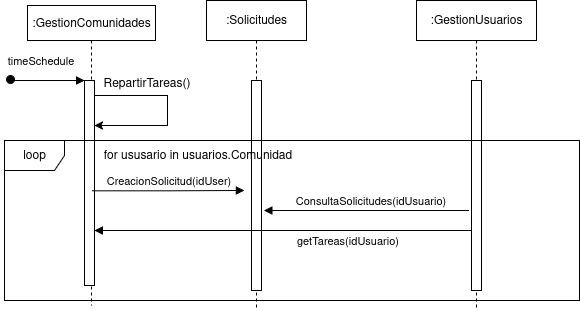
\includegraphics[width=\textwidth]{fotos/6-secuencia.png}
    \caption{Diagrama de secuencia repartir tareas.}
    \label{fig:diagrama_arquitectura}
\end{figure}
\begin{figure}[H]
    \centering
    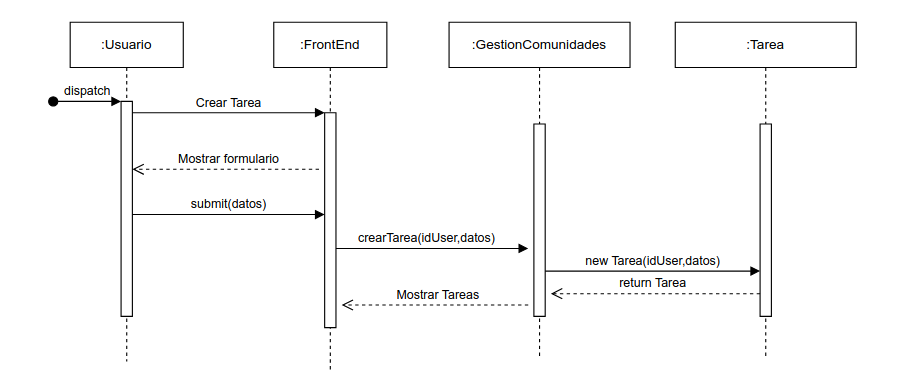
\includegraphics[width=\textwidth]{fotos/final-secuencia.png}
    \caption{Diagrama de secuencia crear tarea.}
    \label{fig:diagrama_arquitectura}
\end{figure}

\newpage

\section{Diseño de la interfaz de usuario}
A continuación, se presentarán los distintos bocetos que compondrán la parte visual del sistema realizando una descripción y análisis de sus características.

\subsection{Landing}
\begin{figure}[H]
    \centering
    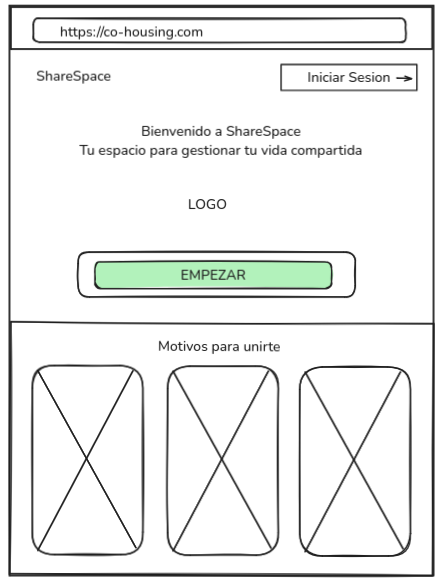
\includegraphics[width=0.5\textwidth]{fotos/Landing-boceto.png}
    \caption{Boceto de la Landing Page.}
    \label{fig:landing-boceto}
\end{figure}
\subsubsection{Descripción}
La interfaz del Landing muestra una pantalla de presentación al usuario de la aplicación, en ella de forma visual se permitirá iniciar sesión o registrarse mostrando además, distintos motivos por los que unirse a la aplicación. Los botones 'Empezar' e 'Iniciar Sesión' actuan como un acceso directo a la sección del Login y Registro.

\subsubsection{Elementos de la interfaz}
\begin{itemize}
  \item Campo de texto con el nombre de la app y mensaje de bienvenida.
  \item Logo.
  \item Botón para Iniciar Sesión.
  \item Botón para Registrarse.
  \item Lista de tarjetas con motivos para unirse.
\end{itemize}

\subsubsection{Funcionalidad}
El usuario puede entender de forma sencilla las distintas características que ofrece la aplicación. Además, le permitirá acceder rápidamente tanto al inicio de sesión como al registro. En general, su funcionalidad es dar una imagen de presentación al usuario de la aplicación.

\subsubsection{Criterios de usabilidad}
\begin{itemize}
  \item La información debe presentarse de forma clara, con una jerarquía visual intuitiva.
  \item Los botones deben ser accesibles, estar correctamente etiquetados y ser fácilmente accionables tanto con ratón como con teclado.
  \item La interfaz debe ser completamente responsive, adaptándose a distintos tamaños de pantalla.
\end{itemize}

\subsection{Login}
\begin{figure}[H]
    \centering
    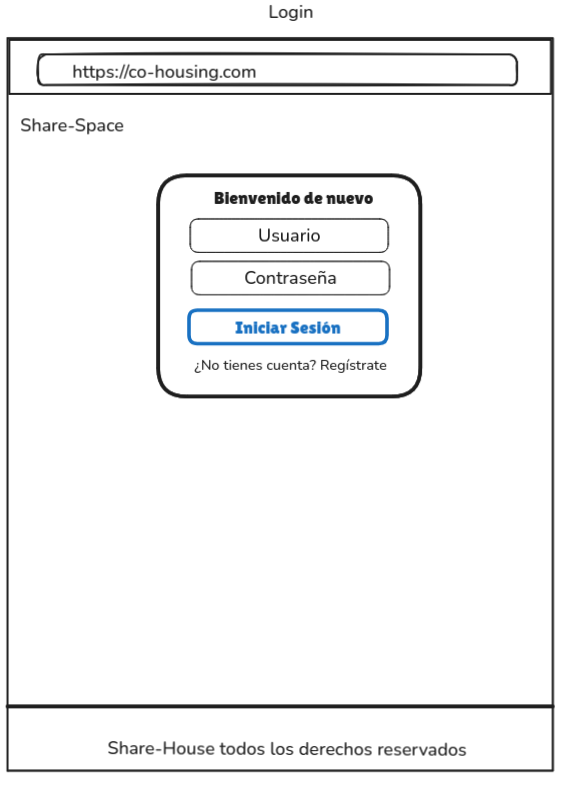
\includegraphics[width=0.5\textwidth]{fotos/login-boceto.png}
    \caption{Boceto del login.}
    \label{fig:login-boceto}
\end{figure}
\subsubsection{Descripción}
Esta interfaz corresponde a la pantalla de inicio de sesión de la aplicación. Su propósito es permitir que el usuario se autentique.

\subsubsection*{Elementos de la interfaz}
\begin{itemize}
  \item Campo de texto para el nombre de usuario.
  \item Campo de texto para la contraseña (con ocultación de caracteres).
  \item Botón de acción para iniciar sesión.
\end{itemize}

\subsubsection{Funcionalidad}
La interfaz permite al usuario introducir su nombre de usuario y contraseña. Al pulsar el botón de inicio de sesión, el sistema valida las credenciales. Si la autenticación es exitosa, el usuario será redirigido a la pantalla principal (Home) de la aplicación. En caso contrario, se mostrará un mensaje de error informando de la autenticación fallida.

\subsubsection{Criterios de usabilidad}
\begin{itemize}
  \item Los campos de entrada deben ser claramente visibles y estar correctamente etiquetados.
  \item El formulario debe proporcionar retroalimentación inmediata en caso de errores, como credenciales inválidas.
  \item El diseño debe ser accesible e intuitivo, permitiendo una navegación fluida desde el teclado y adaptándose a distintos tamaños de pantalla.
\end{itemize}

\subsection{Registro}
\begin{figure}[H]
    \centering
    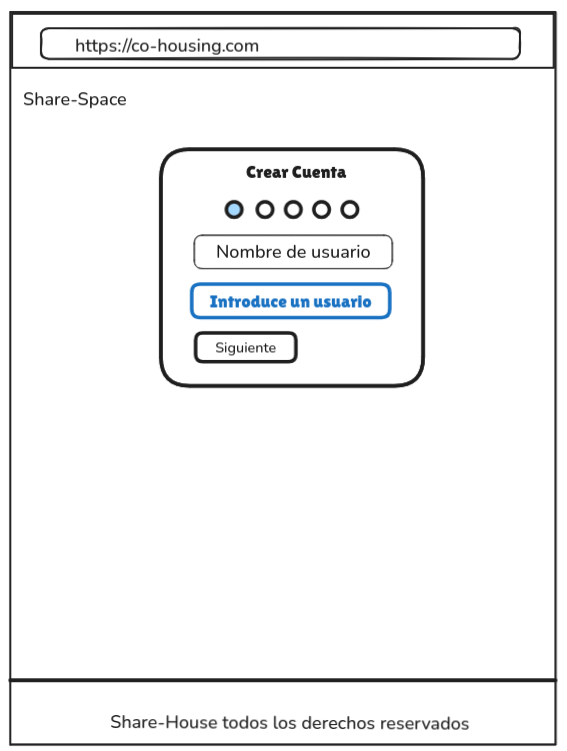
\includegraphics[width=0.5\textwidth]{fotos/registro-boceto.png}
    \caption{Boceto del registro.}
    \label{fig:registro}
\end{figure}
\begin{figure}[H]
    \centering
    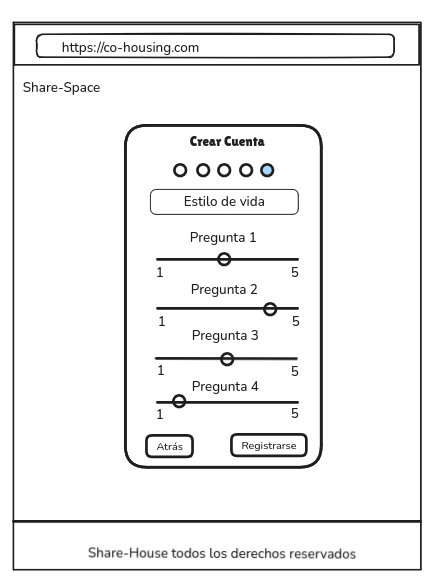
\includegraphics[width=0.5\textwidth]{fotos/registro2-boceto.png}
    \caption{Boceto del registro selección de preferencias.}
    \label{fig:registro2}
\end{figure}
\subsubsection{Descripción}
Esta interfaz corresponde a la pantalla de registro de la aplicación. Su propósito es permitir que el usuario se registre introduciendo sus datos personales y preferencias.

\subsubsection{Elementos de la interfaz}
\begin{itemize}
  \item Una tarjeta que va variando para cada paso del registro.
  \item Campo de texto para introducir credenciales.
  \item Campo seleccionable para introducir el valor de los gustos.
  \item Botón de acción para ir al siguiente paso.
\end{itemize}

\subsubsection{Funcionalidad}
La interfaz permite al usuario introducir sus datos personales y sus gustos. Al pulsar el botón de siguiente, el sistema muestra el siguiente campo, así hasta llegar al final. El último campo es el de los gustos personalizados y será establecido con un selector. Si el registro es exitoso, el usuario será redirigido a la pantalla principal (Home) de la aplicación. En caso contrario, se mostrará un mensaje de error informando del error del registro.

\subsubsection{Criterios de usabilidad}
\begin{itemize}
  \item Los campos de entrada deben ser claramente visibles y estar correctamente etiquetados.
  \item El formulario debe proporcionar retroalimentación inmediata en caso de errores, como credenciales inválidas.
  \item El diseño debe ser accesible e intuitivo, permitiendo una navegación fluida desde el teclado y adaptándose a distintos tamaños de pantalla.
\end{itemize}
\subsection{Home}
\begin{figure}[H]
    \centering
    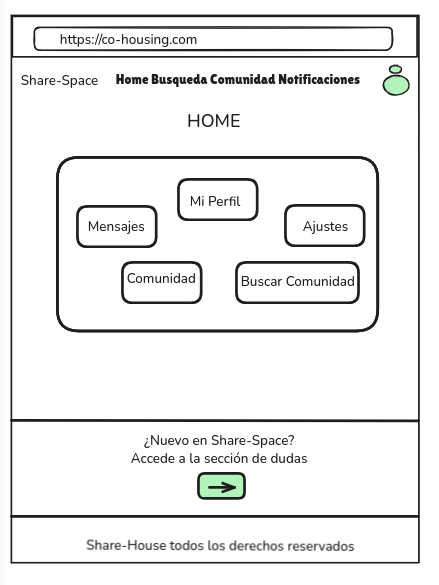
\includegraphics[width=0.5\textwidth]{fotos/Home-boceto.png}
    \caption{Boceto del home.}
    \label{fig:home}
\end{figure}
\subsubsection{Descripción}
La interfaz de inicio (pantalla Home) es la primera vista que el usuario ve tras autenticarse correctamente. Su objetivo es mostrar de forma visual y organizada las distintas funcionalidades que ofrece la aplicación, permitiendo un acceso rápido e intuitivo a cada una de ellas.

\subsubsection{Elementos de la interfaz}
\begin{itemize}
  \item Una tarjeta contenedora que agrupa visualmente todas las funcionalidades disponibles.
  \item Una tarjeta individual por cada funcionalidad, que incluye su nombre y diseño distintivo.
  \item Un botón específico para acceder a la sección de dudas o ayuda.
\end{itemize}

\subsubsection{Funcionalidad}
El usuario puede interactuar con las distintas tarjetas funcionales. Al hacer clic sobre una tarjeta, se le redirige a la sección correspondiente de la aplicación. Asimismo, al pulsar el botón de dudas, el sistema lleva al usuario a la sección de ayuda, donde puede resolver preguntas frecuentes o contactar con soporte.

\subsubsection{Criterios de usabilidad}
\begin{itemize}
  \item Las funcionalidades deben estar claramente identificadas mediante texto y/o iconografía.
  \item Las tarjetas deben ser fácilmente seleccionables, tanto por ratón como por teclado.
  \item El diseño debe ser responsivo y adaptarse a diferentes dispositivos y tamaños de pantalla.
  \item La interfaz debe proporcionar una experiencia de navegación fluida y accesible para todo tipo de usuarios.
\end{itemize}
\subsection{Home de la Comunidad}
\begin{figure}[H]
    \centering
    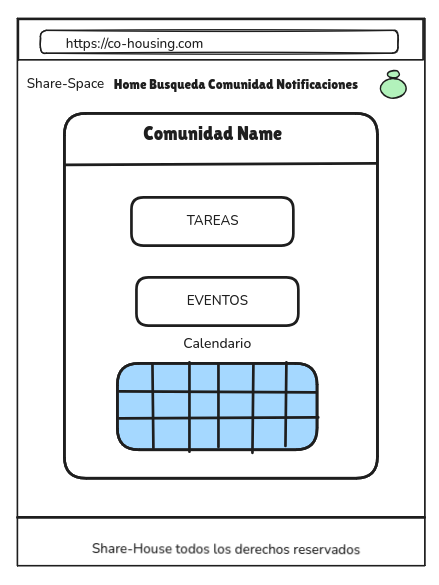
\includegraphics[width=0.5\textwidth]{fotos/tareas-boceto.png}
    \caption{Boceto del home de la comunidad.}
    \label{fig:tareas}
\end{figure}
\subsubsection{Descripción}
La interfaz del Home de la Comunidad permite al usuario visualizar y acceder de forma organizada a las tareas y eventos asignados dentro de la comunidad. Asimismo, integra un calendario interactivo que muestra de manera clara y estructurada todas las actividades asociadas al usuario.

\subsubsection{Elementos de la interfaz}
\begin{itemize}
  \item Tarjeta de acceso a las tareas asignadas al usuario dentro de la comunidad.
  \item Tarjeta de acceso a los eventos en los que el usuario participa.
  \item Calendario interactivo que muestra visualmente las tareas y eventos programados.
\end{itemize}

\subsubsection{Funcionalidad}
El usuario puede interactuar con las distintas tarjetas funcionales para acceder a secciones específicas:
\begin{itemize}
  \item Al seleccionar la tarjeta de tareas, se accede al listado detallado de actividades que debe realizar.
  \item Al seleccionar la tarjeta de eventos, se muestran los eventos comunitarios en los que está inscrito.
  \item El calendario ofrece una vista global donde se reflejan las tareas y eventos del usuario, facilitando su planificación y seguimiento.
\end{itemize}

\subsubsection{Criterios de usabilidad}
\begin{itemize}
  \item Cada elemento funcional debe estar claramente identificado mediante texto e iconografía representativa.
  \item La interfaz debe ser completamente navegable mediante teclado y compatible con tecnologías de asistencia.
  \item El diseño debe adaptarse correctamente a distintos dispositivos (responsive design).
  \item Las interacciones deben ser intuitivas, con retroalimentación visual ante acciones del usuario (hover, selección, etc.).
\end{itemize}


\subsection{Tareas}
\begin{figure}[H]
    \centering
    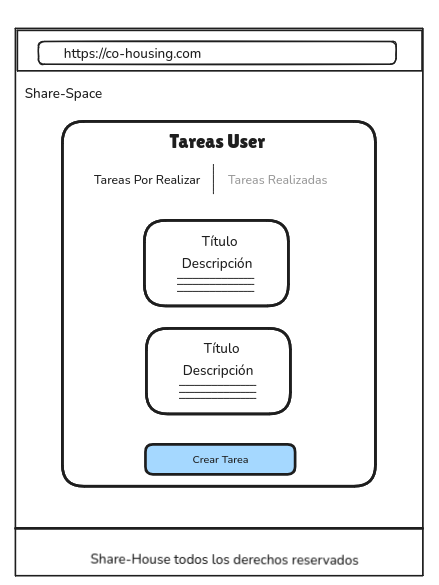
\includegraphics[width=0.5\textwidth]{fotos/lista-tareas.png}
    \caption{Boceto de la lista de tareas del usuario.}
    \label{fig:tareas}
\end{figure}
\subsubsection{Descripción}
La interfaz de la lista de tareas permite al usuario ver todas las tareas que tiene asignado en esta semana, aquí se mostrará una tarjeta para cada tarea mostrando el título y su descripción. Las tareas mostradas se dividirán en dos listas diferentes: las que están por realizar y las realizadas. Finalmente contiene un botón que redirecciona a un formulario para crear Tarea.

\subsubsection{Elementos de la interfaz}
\begin{itemize}
  \item Tarjeta con la información principal de cada Tarea, si se pulsa la tarjeta redirecciona al perfil de la tarea.
  \item Botón para crear Tarea.
  \item Campo de texto con la descripción detallada de la tarea.
  \item Filtro de tareas realizadas y por realizar.
\end{itemize}

\subsubsection{Funcionalidad}
El usuario puede:
\begin{itemize}
  \item Consultar todas las tareas asignadas en esta semana
  \item Crear una nueva tarea
  \item Pulsar la tarjeta para acceder al perfil de una tarea
\end{itemize}

\subsubsection{Criterios de usabilidad}
\begin{itemize}
  \item Los botones y elementos interactivos deben ser fácilmente identificables y tener etiquetas comprensibles.
  \item El diseño debe ser adaptable a distintos tamaños de pantalla, priorizando la usabilidad en dispositivos móviles.
\end{itemize}

\subsection{Tarea Específica}
\begin{figure}[H]
    \centering
    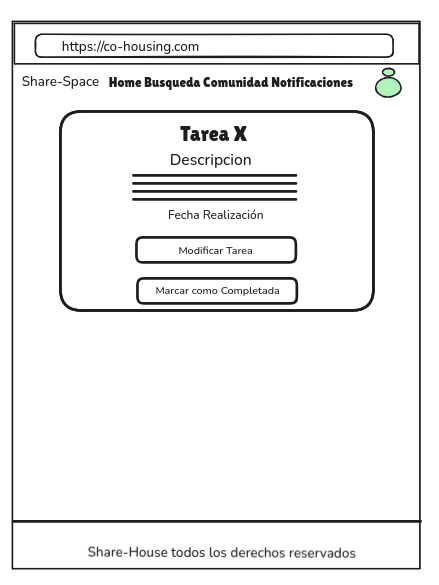
\includegraphics[width=0.5\textwidth]{fotos/Tarea-boceto.png}
    \caption{Boceto de la tarea.}
    \label{fig:home}
\end{figure}


\subsubsection{Descripción}
La interfaz de visualización de Tarea específica permite al usuario consultar la información detallada de una tarea concreta. Funciona como un perfil individual de la tarea, mostrando su título, descripción, fecha límite de realización y un botón para modificar la tarea, que redirige a un formulario de edición.

\subsubsection{Elementos de la interfaz}
\begin{itemize}
  \item Tarjeta principal que agrupa toda la información de la tarea.
  \item Campo de texto con el título de la tarea.
  \item Campo de texto con la descripción detallada de la tarea.
  \item Fecha límite (fecha tope) de realización claramente visible.
  \item Botón de modificación que redirecciona al formulario de edición.
  \item Botón para marcar la tarea como completada.
\end{itemize}

\subsubsection{Funcionalidad}
El usuario puede:
\begin{itemize}
  \item Consultar todos los detalles relevantes de una tarea específica.
  \item Ver la fecha límite para su realización.
  \item Pulsar el botón de edición para modificar la información de la tarea, siendo redirigido al formulario correspondiente.
  \item Pulsar el botón de completada, para marcar una tarea como finalizada.
\end{itemize}

\subsubsection{Criterios de usabilidad}
\begin{itemize}
  \item Los botones deben ser visibles y accesibles.
  \item El diseño debe garantizar la legibilidad de los campos.
\end{itemize}


\subsection{Buscador de comunidades}
\begin{figure}[H]
    \centering
    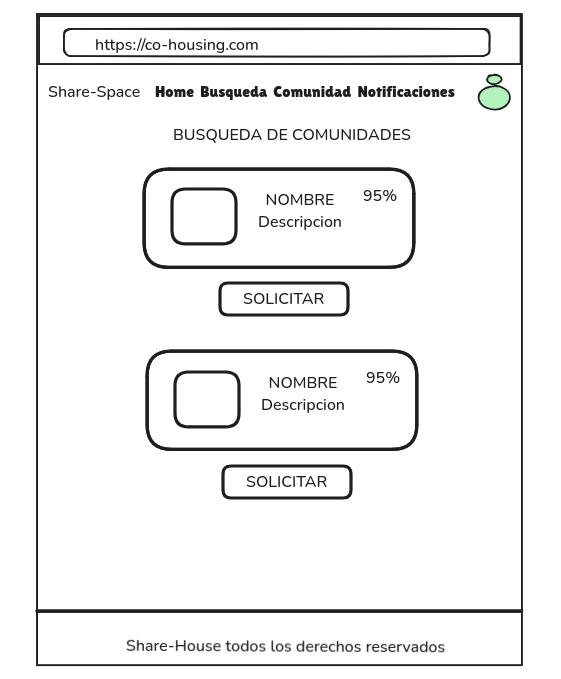
\includegraphics[width=0.5\textwidth]{fotos/Busqueda-boceto.png}
    \caption{Boceto de la sección de búsqueda.}
    \label{fig:busqueda}
\end{figure}

\subsubsection{Descripción}
La interfaz de búsqueda de comunidades afines muestra al usuario un listado de comunidades recomendadas en función de su afinidad. Cada comunidad se presenta mediante una tarjeta que incluye su imagen principal, nombre, descripción y el porcentaje de afinidad calculado. Además, se incluye un botón que permite al usuario solicitar unirse a dicha comunidad.

\subsubsection{Elementos de la interfaz}
\begin{itemize}
  \item Tarjeta principal que agrupa la información visual de cada comunidad sugerida.
  \item Imagen representativa de la comunidad.
  \item Campo de texto con el nombre de la comunidad.
  \item Descripción resumida de la comunidad.
  \item Indicador del porcentaje de afinidad entre el usuario y la comunidad.
  \item Botón de acción para solicitar la unión a la comunidad.
\end{itemize}

\subsubsection{Funcionalidad}
El usuario puede explorar visualmente las distintas comunidades sugeridas, revisando su información básica y valorando su grado de afinidad. Si desea formar parte de una comunidad concreta, puede pulsar el botón de "Solicitar unión", lo que enviará una solicitud al sistema o a los administradores de dicha comunidad.

\subsubsection{Criterios de usabilidad}
\begin{itemize}
  \item Los botones de acción deben ser fácilmente reconocibles y estar bien etiquetados.
  \item La interfaz debe ser adaptable a distintos dispositivos (responsive), asegurando la legibilidad y usabilidad.
\end{itemize}


\subsection{Perfil del usuario}
\begin{figure}[H]
    \centering
    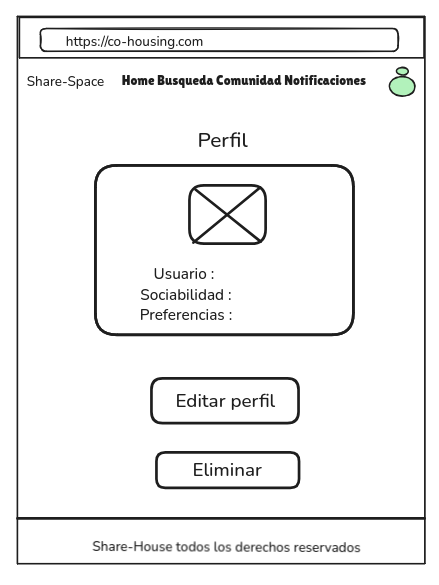
\includegraphics[width=0.5\textwidth]{fotos/perfil-usuario-boceto.png}
    \caption{Boceto del perfil del usuario.}
    \label{fig:perfil-user}
\end{figure}
\subsubsection{Descripción}
La interfaz del perfil de usuario permite visualizar y gestionar los datos personales del usuario. En esta vista se muestran su avatar, nombre de usuario y los criterios de afinidad o gustos que ha definido. Además, se incluyen dos botones de acción: uno para acceder al formulario de edición del perfil y otro para eliminar la cuenta de usuario.

\subsubsection{Elementos de la interfaz}
\begin{itemize}
  \item Tarjeta principal que agrupa la información visual del usuario.
  \item Imagen (avatar) del usuario.
  \item Campo de texto con el nombre de usuario.
  \item Visualización de los criterios de afinidad o gustos del usuario.
  \item Botón para acceder al formulario de edición del perfil.
  \item Botón para eliminar el perfil del usuario.
\end{itemize}

\subsubsection{Funcionalidad}
El usuario puede consultar de forma clara la información de su perfil, incluyendo su imagen, nombre y preferencias personales. Asimismo, se proporcionan opciones para modificar estos datos o eliminar su cuenta mediante los botones de edición y eliminación, respectivamente.

\subsubsection{Criterios de usabilidad}
\begin{itemize}
  \item Los botones deben ser accesibles, estar bien etiquetados y ser fácilmente accionables.
  \item La interfaz debe ser completamente responsive, adaptándose a distintos tamaños de pantalla.

\end{itemize}

\subsection{Solicitudes}
\begin{figure}[H]
    \centering
    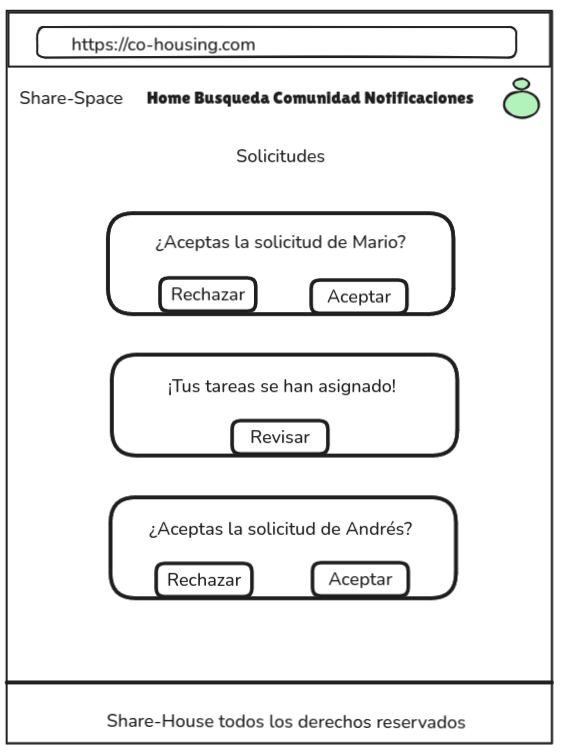
\includegraphics[width=0.5\textwidth]{fotos/Solicitudes-boceto.png}
    \caption{Boceto de la sección de Solicitudes.}
    \label{fig:solicitudes}
\end{figure}
\subsubsection{Descripción}
La interfaz de solicitudes muestra todas las solicitudes pendientes del usuario, incluyendo el mensaje de la solicitud y el nombre del remitente. Para cada solicitud, se presentan tres opciones mediante botones: aceptar, rechazar o revisar. El botón 'revisar' actúa como un acceso directo a secciones relacionadas, como tareas asignadas.

\subsubsection{Elementos de la interfaz}
\begin{itemize}
  \item Tarjetas individuales para cada una de las solicitudes.
  \item Campo de texto con la descripción de la solicitud.
  \item Botón para aceptar la solicitud.
  \item Botón para rechazar la solicitud.
  \item Botón para revisar tareas o ver detalles de la comunidad, que redirecciona a otra sección.
\end{itemize}

\subsubsection{Funcionalidad}
El usuario puede visualizar todas las solicitudes pendientes y leer sus descripciones. Puede interactuar con ellas mediante los botones de aceptar, rechazar o revisar. Al realizar cualquiera de estas acciones, la solicitud correspondiente desaparece de la lista.

\subsubsection{Criterios de usabilidad}
\begin{itemize}
  \item La información debe presentarse de forma clara, con una jerarquía visual intuitiva.
  \item Los botones deben ser accesibles, estar correctamente etiquetados y ser fácilmente accionables tanto con ratón como con teclado.
  \item La interfaz debe ser completamente responsive, adaptándose a distintos tamaños de pantalla.

\end{itemize}

\section{Diagrama de navegabilidad}
Para poder entender como va a ser el flujo de navegabilidad por las distintas pantallas de la aplicación se ha realizado el siguiente diagrama.
\begin{figure}[H]
    \centering
    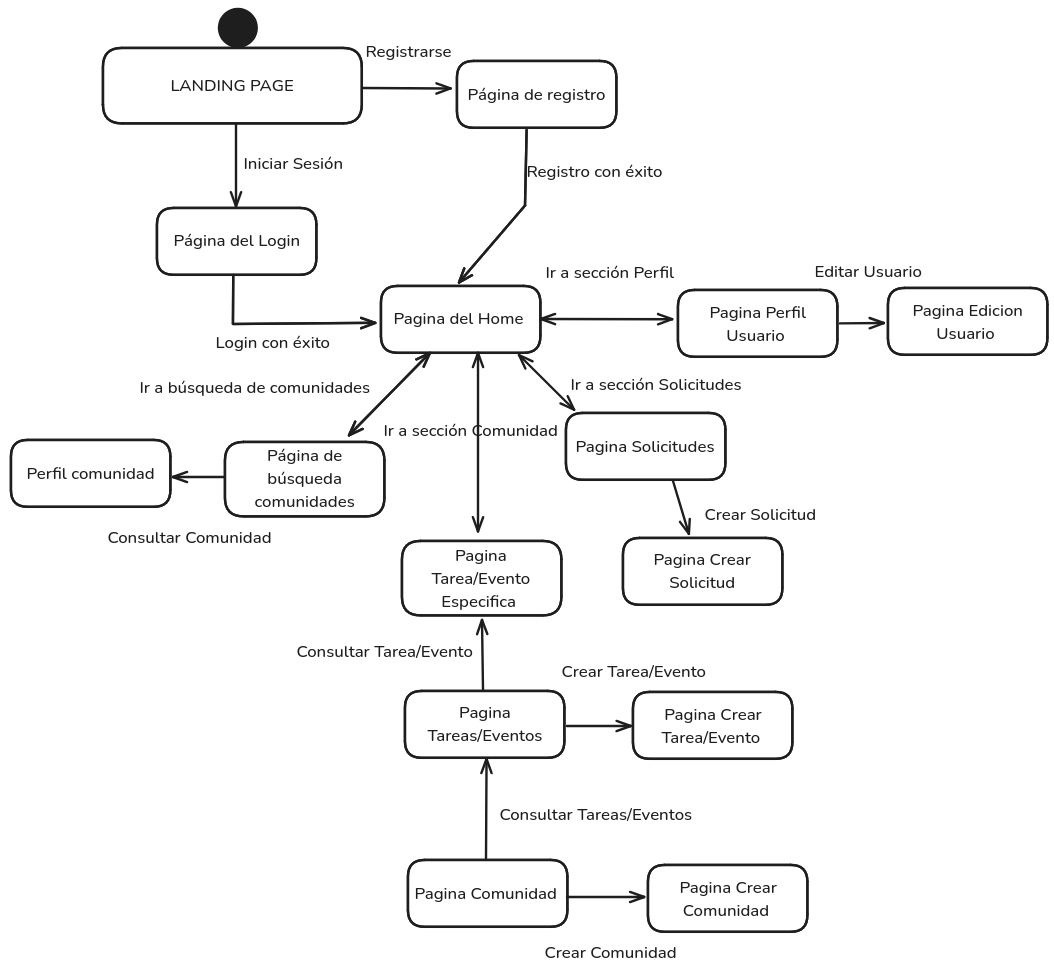
\includegraphics[width=1\textwidth]{fotos/diagramaNavegabilidad.png}
    \caption{Diagrama de navegabilidad del sistema.}
    \label{fig:mapa-navegabilidad}
\end{figure}

